\noindent
En esta sección se resumen los fundamentos teóricos necesarios para el resto del trabajo. Se presentan el modelo de cámara, homografías para el plano del suelo, y los operadores de detección de bordes y líneas, así como la notación homogénea para rectas y el concepto de puntos de fuga.

\subsubsection{Modelo de cámara pinhole y calibración}\label{subsec:camera}
\noindent
El modelo pinhole aproxima la formación de imagen como una proyección central desde el centro óptico al plano de imagen. Bajo esta aproximación, un punto del mundo en el plano del suelo (aproximadamente coplanar) se proyecta mediante una transformación proyectiva. La calibración intrínseca estima la matriz de cámara y la distorsión, permitiendo normalizar coordenadas y razonar geométricamente con menor sesgo \cite{hartley2003multiple}.

\subsubsection{Homografías en el plano del suelo}\label{subsec:homografias}
\noindent
Cuando los puntos pertenecen a un mismo plano (p. ej., el asfalto),
la relación entre sus proyecciones en dos vistas o entre el plano del mundo
y la imagen puede modelarse con una homografía
\(\mathbf{H}\in\mathbb{R}^{3\times3}\)
definida a escala \cite{hartley2003multiple}.
Esta matriz permite mapear cuadriláteros en la imagen a cuadrados canónicos,
facilitando medir y extrapolar una retícula en la imagen.

\subsubsection{Bordes y líneas: Canny y Hough}\label{sec:canny-hough}
\noindent
La extracción de bordes con Canny proporciona contornos estables frente a ruido mediante suavizado, gradiente y supresión no máxima \cite{canny1986edge}. La transformada de Hough detecta rectas parametrizando \(\rho,\theta\) y acumulando votos para evidenciar alineamientos \cite{ballard1981hough}. Estas dos herramientas permiten obtener segmentos candidatos a las marcas viales de la retícula.

\subsubsection{Rectas en coordenadas homogéneas y SVD}\label{sec:rectas-svd}
\noindent
Una recta en la imagen se representa como \(\ell=[A,B,C]^\top\) tal que \(\ell^\top\,\mathbf{x}=0\) para puntos homogéneos \(\mathbf{x}=[x,y,1]^\top\). Dadas dos observaciones \((x_i,y_i)\), resolver \(\mathbf{M}\,[A\ B\ C]^\top=\mathbf{0}\) con \(\mathbf{M}=\begin{bmatrix}x_1&y_1&1\\x_2&y_2&1\end{bmatrix}\) produce \(\ell\) como vector del espacio nulo. La SVD ofrece un procedimiento robusto para obtener dicho vector \cite{golub2013matrix}. Las intersecciones entre rectas se obtienen con el producto cruz \(\mathbf{x}=\ell_1\times\ell_2\) y se deshomogeneizan si \(x_3\neq 0\).

\subsubsection{Intersecciones de líneas y \textit{clustering}}\label{sec:intersections-clustering}
\noindent
Dados conjuntos de rectas \(\{\ell_i\}\) en coordenadas homogéneas, las intersecciones puntuales se calculan con el producto cruz
\(\mathbf{x}_{ij} = \ell_i \times \ell_j\). Si \(x_{ij,3} \neq 0\), el punto es finito y se deshomogeneiza como \( (x_{ij}/x_{ij,3},\ y_{ij}/x_{ij,3}) \); valores \(x_{ij,3} \approx 0\) indican intersecciones en el infinito (rectas prácticamente paralelas) \cite{hartley2003multiple}.

\noindent
En escenas urbanas con estructura aproximadamente Manhattan, muchas rectas convergen hacia uno o varios puntos de fuga. Por tanto, las
intersecciones finitas tienden a concentrarse en vecindades cercanas a la línea del horizonte. Un filtrado previo por banda horizontal
reduce ruido: se retienen solo las intersecciones con \(y\) dentro de una franja alrededor del horizonte estimado (Sección~\ref{sec:vanishing-points}).

\noindent
Para consolidar evidencia y atenuar outliers, se agrupan las intersecciones \emph{relevantes} mediante técnicas de \textit{clustering} no supervisado.
Una opción práctica es el \texttt{AgglomerativeClustering} con umbral de distancia para dejar que los datos determinen el número de cúmulos; alternativas
como DBSCAN también son adecuadas cuando existen densidades heterogéneas \cite{tan2005introduction}. Los centroides de los cúmulos proporcionan
estimaciones iniciales de puntos de fuga que luego pueden refinarse por mínimos cuadrados o criterios estadísticamente consistentes
\cite{kanatani1998statistical,hartley2003multiple}.

\noindent
En resumen, el flujo teórico es: (i) estimar rectas, (ii) generar intersecciones por pares, (iii) filtrar por banda cercana al horizonte,
(iv) agrupar por proximidad, y (v) usar los centroides de cúmulos como candidatos a puntos de fuga para la separación de haces de líneas.

\subsubsection{Puntos de fuga}\label{sec:vanishing-points}
\noindent
Cuando proyectamos una escena del mundo real en tres dimensiones sobre un plano bidimensional, 
como la película o el sensor de una cámara, se produce una transformación en la imagen.
Esta transformación, conocida como transformación proyectiva, provoca que las líneas paralelas en el mundo real,
 al proyectarse en el plano de la cámara, se intersecten en un punto denominado punto de fuga.
  La Fig.~\ref{fig:distorion-teo} ilustra el fenómeno de paralelismo en 3D y su proyección en 2D.

\begin{figure}[!ht]
	\centering
	\begin{subfigure}{0.4\textwidth}
		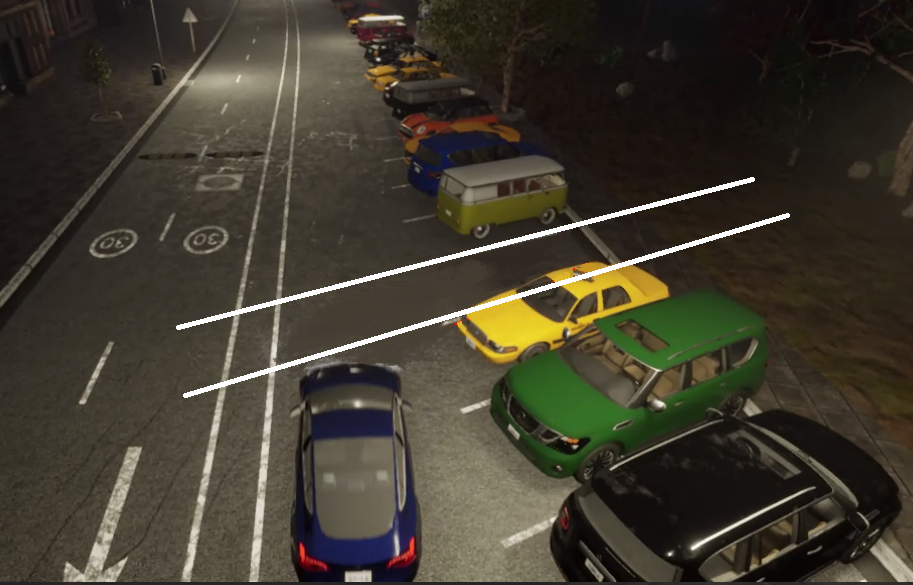
\includegraphics[width=\textwidth]{img/reticule/paralel_lines}
		\caption{Ejemplo de líneas paralelas en un escenario real en tres dimensiones.}
	\end{subfigure}
	\begin{subfigure}{0.4\textwidth}
		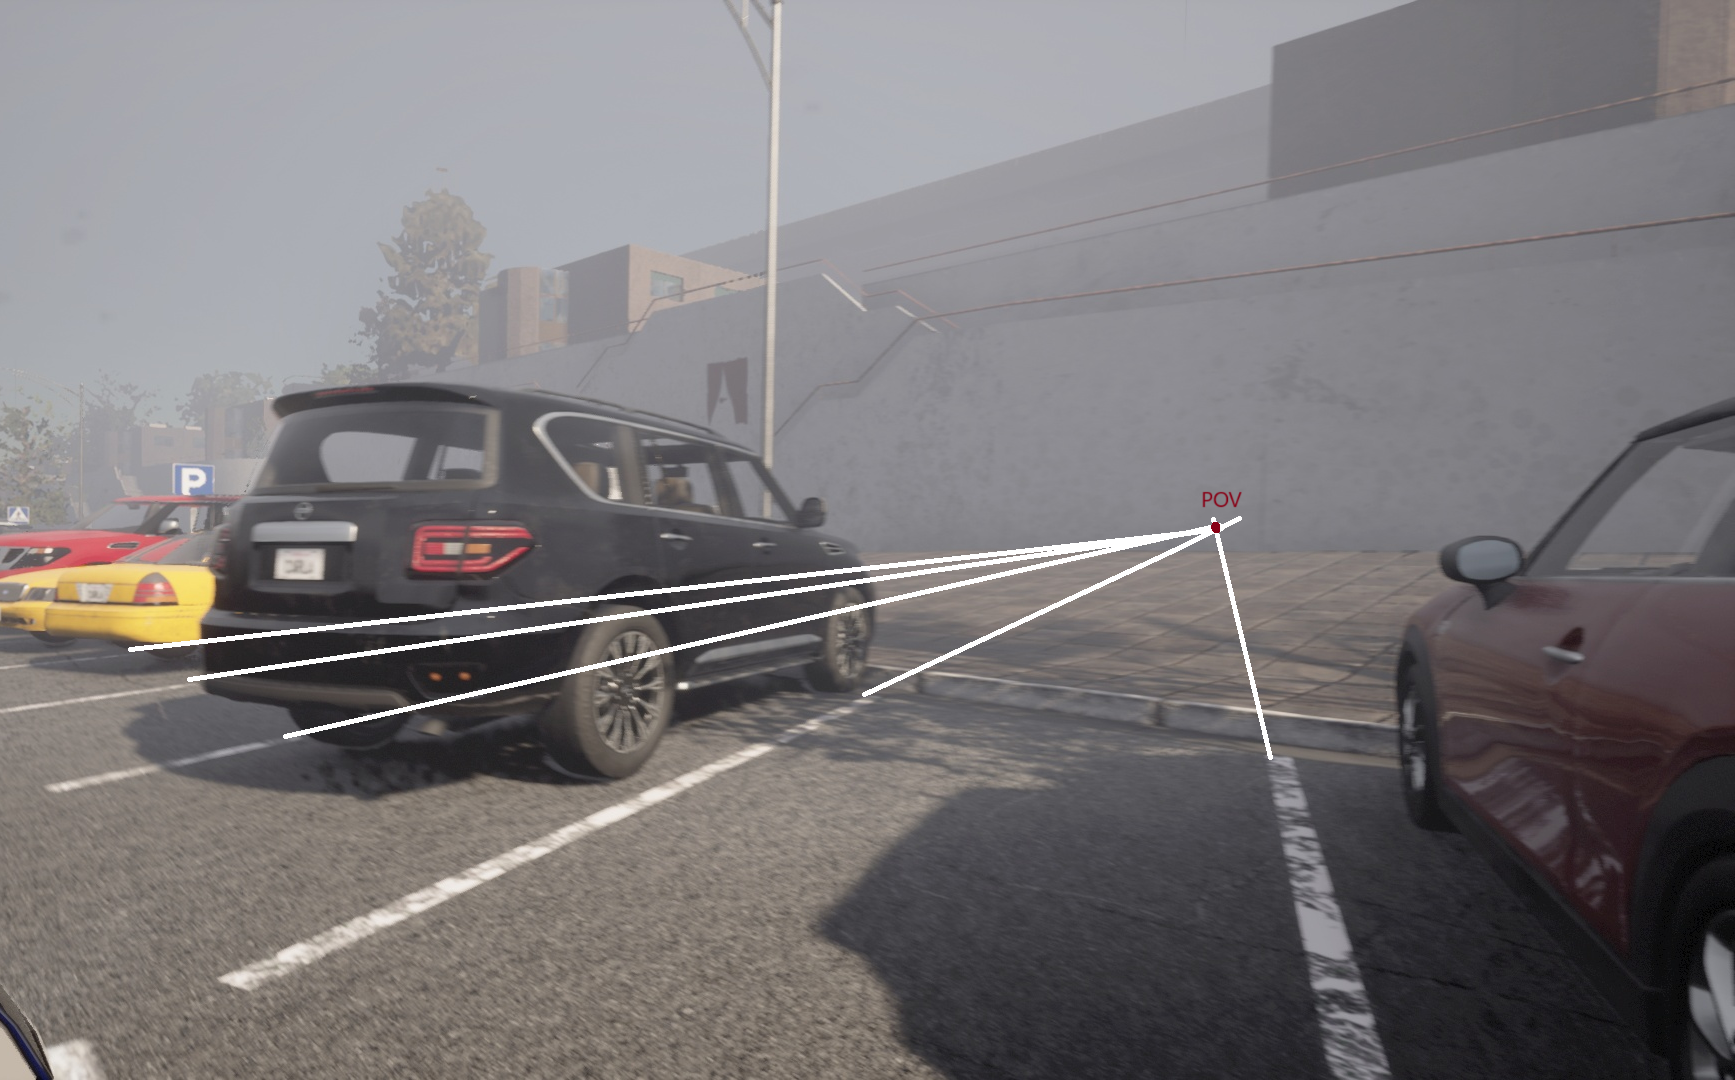
\includegraphics[width=\textwidth]{img/reticule/pov}
		\caption{Proyección de líneas paralelas en el plano de la cámara.}
	\end{subfigure}
	\caption{Paralelismo en 3D y su proyección al plano de imagen.}
	\label{fig:distorion-teo}
\end{figure}

\noindent
Estimar puntos de fuga con múltiples líneas y criterios robustos reduce la sensibilidad a ruido y oclusiones 
\cite{hartley2003multiple,kanatani1998statistical}. En este trabajo se emplean dos puntos de fuga para separar
 las marcas de la retícula en dos conjuntos según su punto de fuga, coherentes con la geometría del estacionamiento.
